In order to reveal the structure of the network $G$, we choose to reorder the matrix.
There are many ways to rearrange a symmetric matrix, Behrisch et al. \cite{behrisch_matrix_2016} provides a good review of those methods.
In practice, we notice that many methods will introduce so called the \emph{Off-diagonal Block Pattern} even when there is no such pattern in the data.
We consider this as an artifact of the algorithms.

We want to reorder the matrix into an approximate block diagonal form, so that all the papers produced by the same group will be arranged close to each other.
We achieve this by minimizing the weighted linear arrangement (LA) loss function:

\begin{equation}
    \textbf{LA}'(G, \pi) = \sum_{ij \in E} w_{i,j} \cdot |\pi(i) - \pi(j)|
\end{equation}

where $\pi$ is a one-to-one function $V \rightarrow \{1,2,\cdots,|V|\}$ representing the permutation of the nodes in 1D, a.k.a the arrangement of the matrix;
$w_{i,j}$ is the weights of the edge between node $i$ and $j$.

In this paper, we use a normalized version of MinLA:
\begin{equation}
    \textbf{LA}(G, \pi) = \sum_{ij \in E} w_{i,j} \cdot \frac{|\pi(i) - \pi(j)|}{|V|^2}
\end{equation}

where $|V|$ is the number of nodes.

This is known as the minimum linear arrangement (MinLA) problem.
The MinLA problem was introduced in 1973 as the \emph{optimal linear ordering problem} \cite{adolphson_optimal_1973}.
It is a special case of the \emph{quadratic assignment problem}, where every node is in a line and have equal unit distance to it's neighbors.
It is proved to be a NP-complete problem \cite{garey_simplified_1976},
One should not expect to solve a large scale NP-complete using exact methods, 
e.g. \cite{andrade_minimum_2017} only works with no more than 20 nodes.
Petit \cite{petit_experiments_2004} has thoroughly introduced some heuristic methods that can provide approximate optimal solutions to the MinLA problem, 
including the hill climbing method.

A basic hill climbing algorithm can be described in Algo. \ref{algo:hillclimbing}. 

\begin{algorithm}
    \caption{Hill Climbing}\label{algo:hillclimbing}
    \begin{algorithmic}[1]
        \State \textbf{while} not Terminated:
        \State \hskip2em $i,j \leftarrow \textbf{random}()$
        \State \hskip2em \textbf{if} \textbf{swapCanReduceLA}(i,j): \Comment{This can be done in $O(|V|)$.}
        \State \hskip4em \textbf{swap}(i,j)
    \end{algorithmic}
\end{algorithm}

To take advantage of the power of parallel computing, we propose a GPU augmented hill climbing method, described in Algo. \ref{algo:gpu_hill_climbing}.

\begin{algorithm}
    \caption{GPU augmented Hill Climbing}\label{algo:gpu_hill_climbing}
    \begin{algorithmic}[1]
        \State \textbf{while} not Terminated:
        \State \hskip2em Detect pairs which if swapped will reduce the LA cost \Comment{With 32,768 threads on GPU}
        \State \hskip2em Sort pairs by the gains (the amount that can be reduced)
        \State \hskip2em Remove conflicted pairs with less gains
        \State \hskip2em Swap all remaining pairs
        \State \hskip2em If number of the found pairs is small:
        \State \hskip4em Double the number of parallel threads for detection until limit hit
    \end{algorithmic}
\end{algorithm}

Fig. \ref{fig:gpu_hill_climbing} shows the comparison of Algo. \ref{algo:hillclimbing} and \ref{algo:gpu_hill_climbing} in wall time.

\begin{figure}
    \centering
    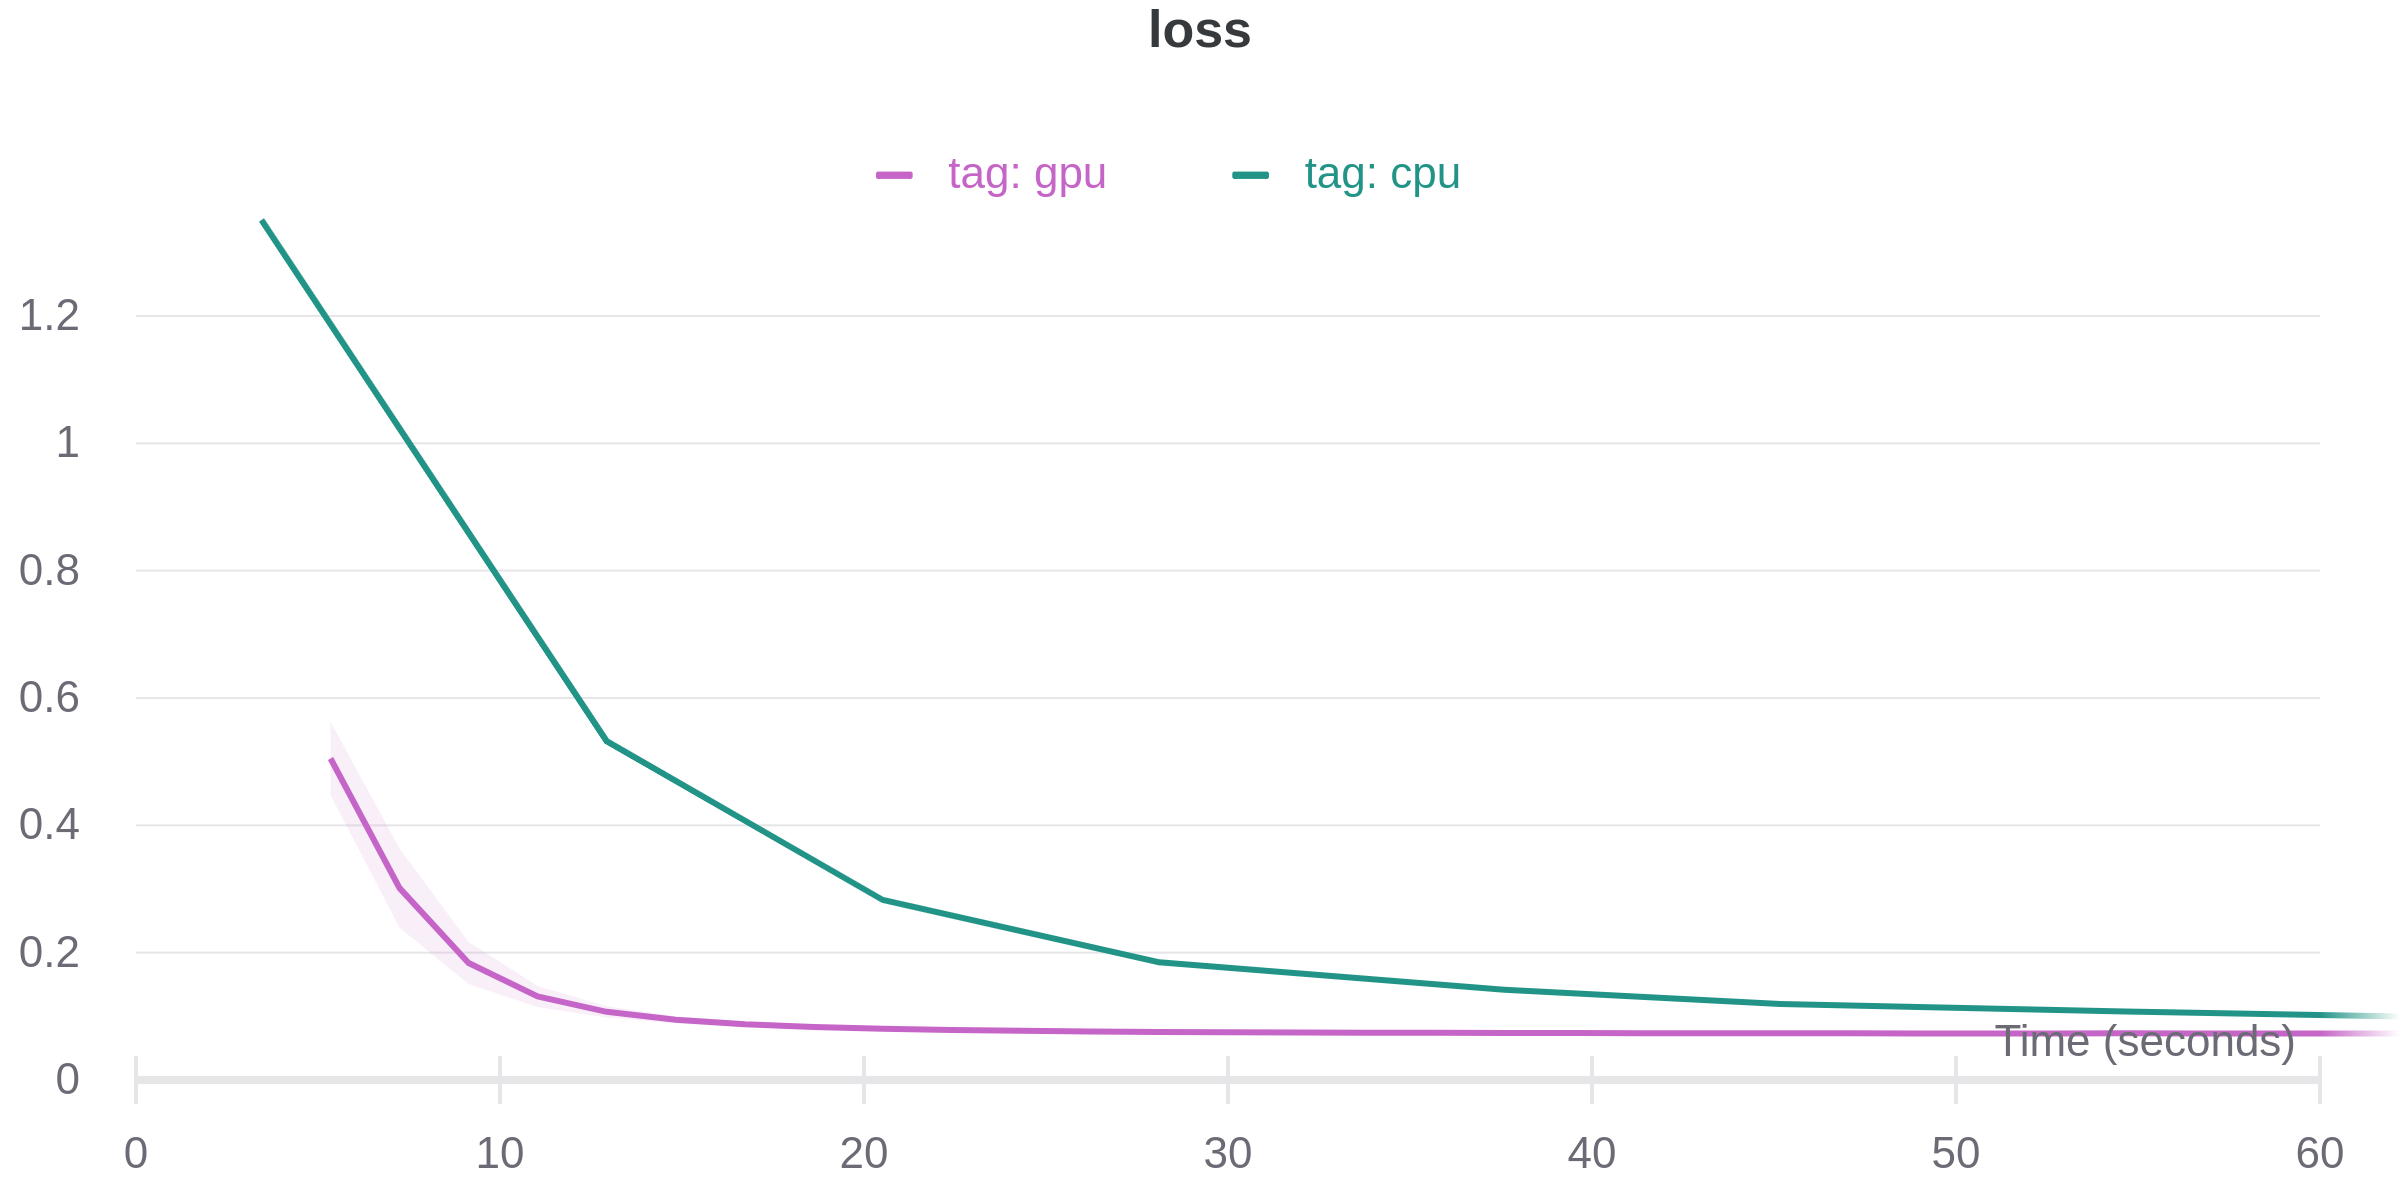
\includegraphics[width=0.8\textwidth]{images/curve_60s.png}
    \caption{A comparison of the first 60 seconds of the optimization curve of Algo. \ref{algo:hillclimbing} and \ref{algo:gpu_hill_climbing}. 
    Averaged over 100 independent runs.
    The GPU augmented algorithm is better than the basic algorithm in wall-clock time.
    }
    \label{fig:gpu_hill_climbing}
\end{figure}

Both the basic hill climbing algorithm and the GPU augmented hill climbing algorithm are implemented in Python and accelerated by Numba \cite{lam_numba_2015}.
One instance of Algo. \ref{algo:hillclimbing} uses one Intel 6230 CPU core.
One instance of Algo. \ref{algo:gpu_hill_climbing} uses one Intel 6130 CPU core and one NVIDIA Tesla V100s GPU.

Both methods are fast enough to get reasonably good results in less than one minute, though the GPU augmented version can achieve better solutions in general.
One of the results can be visualized in Fig. \ref{fig:optimization_results}.

\begin{figure}
    \centering
    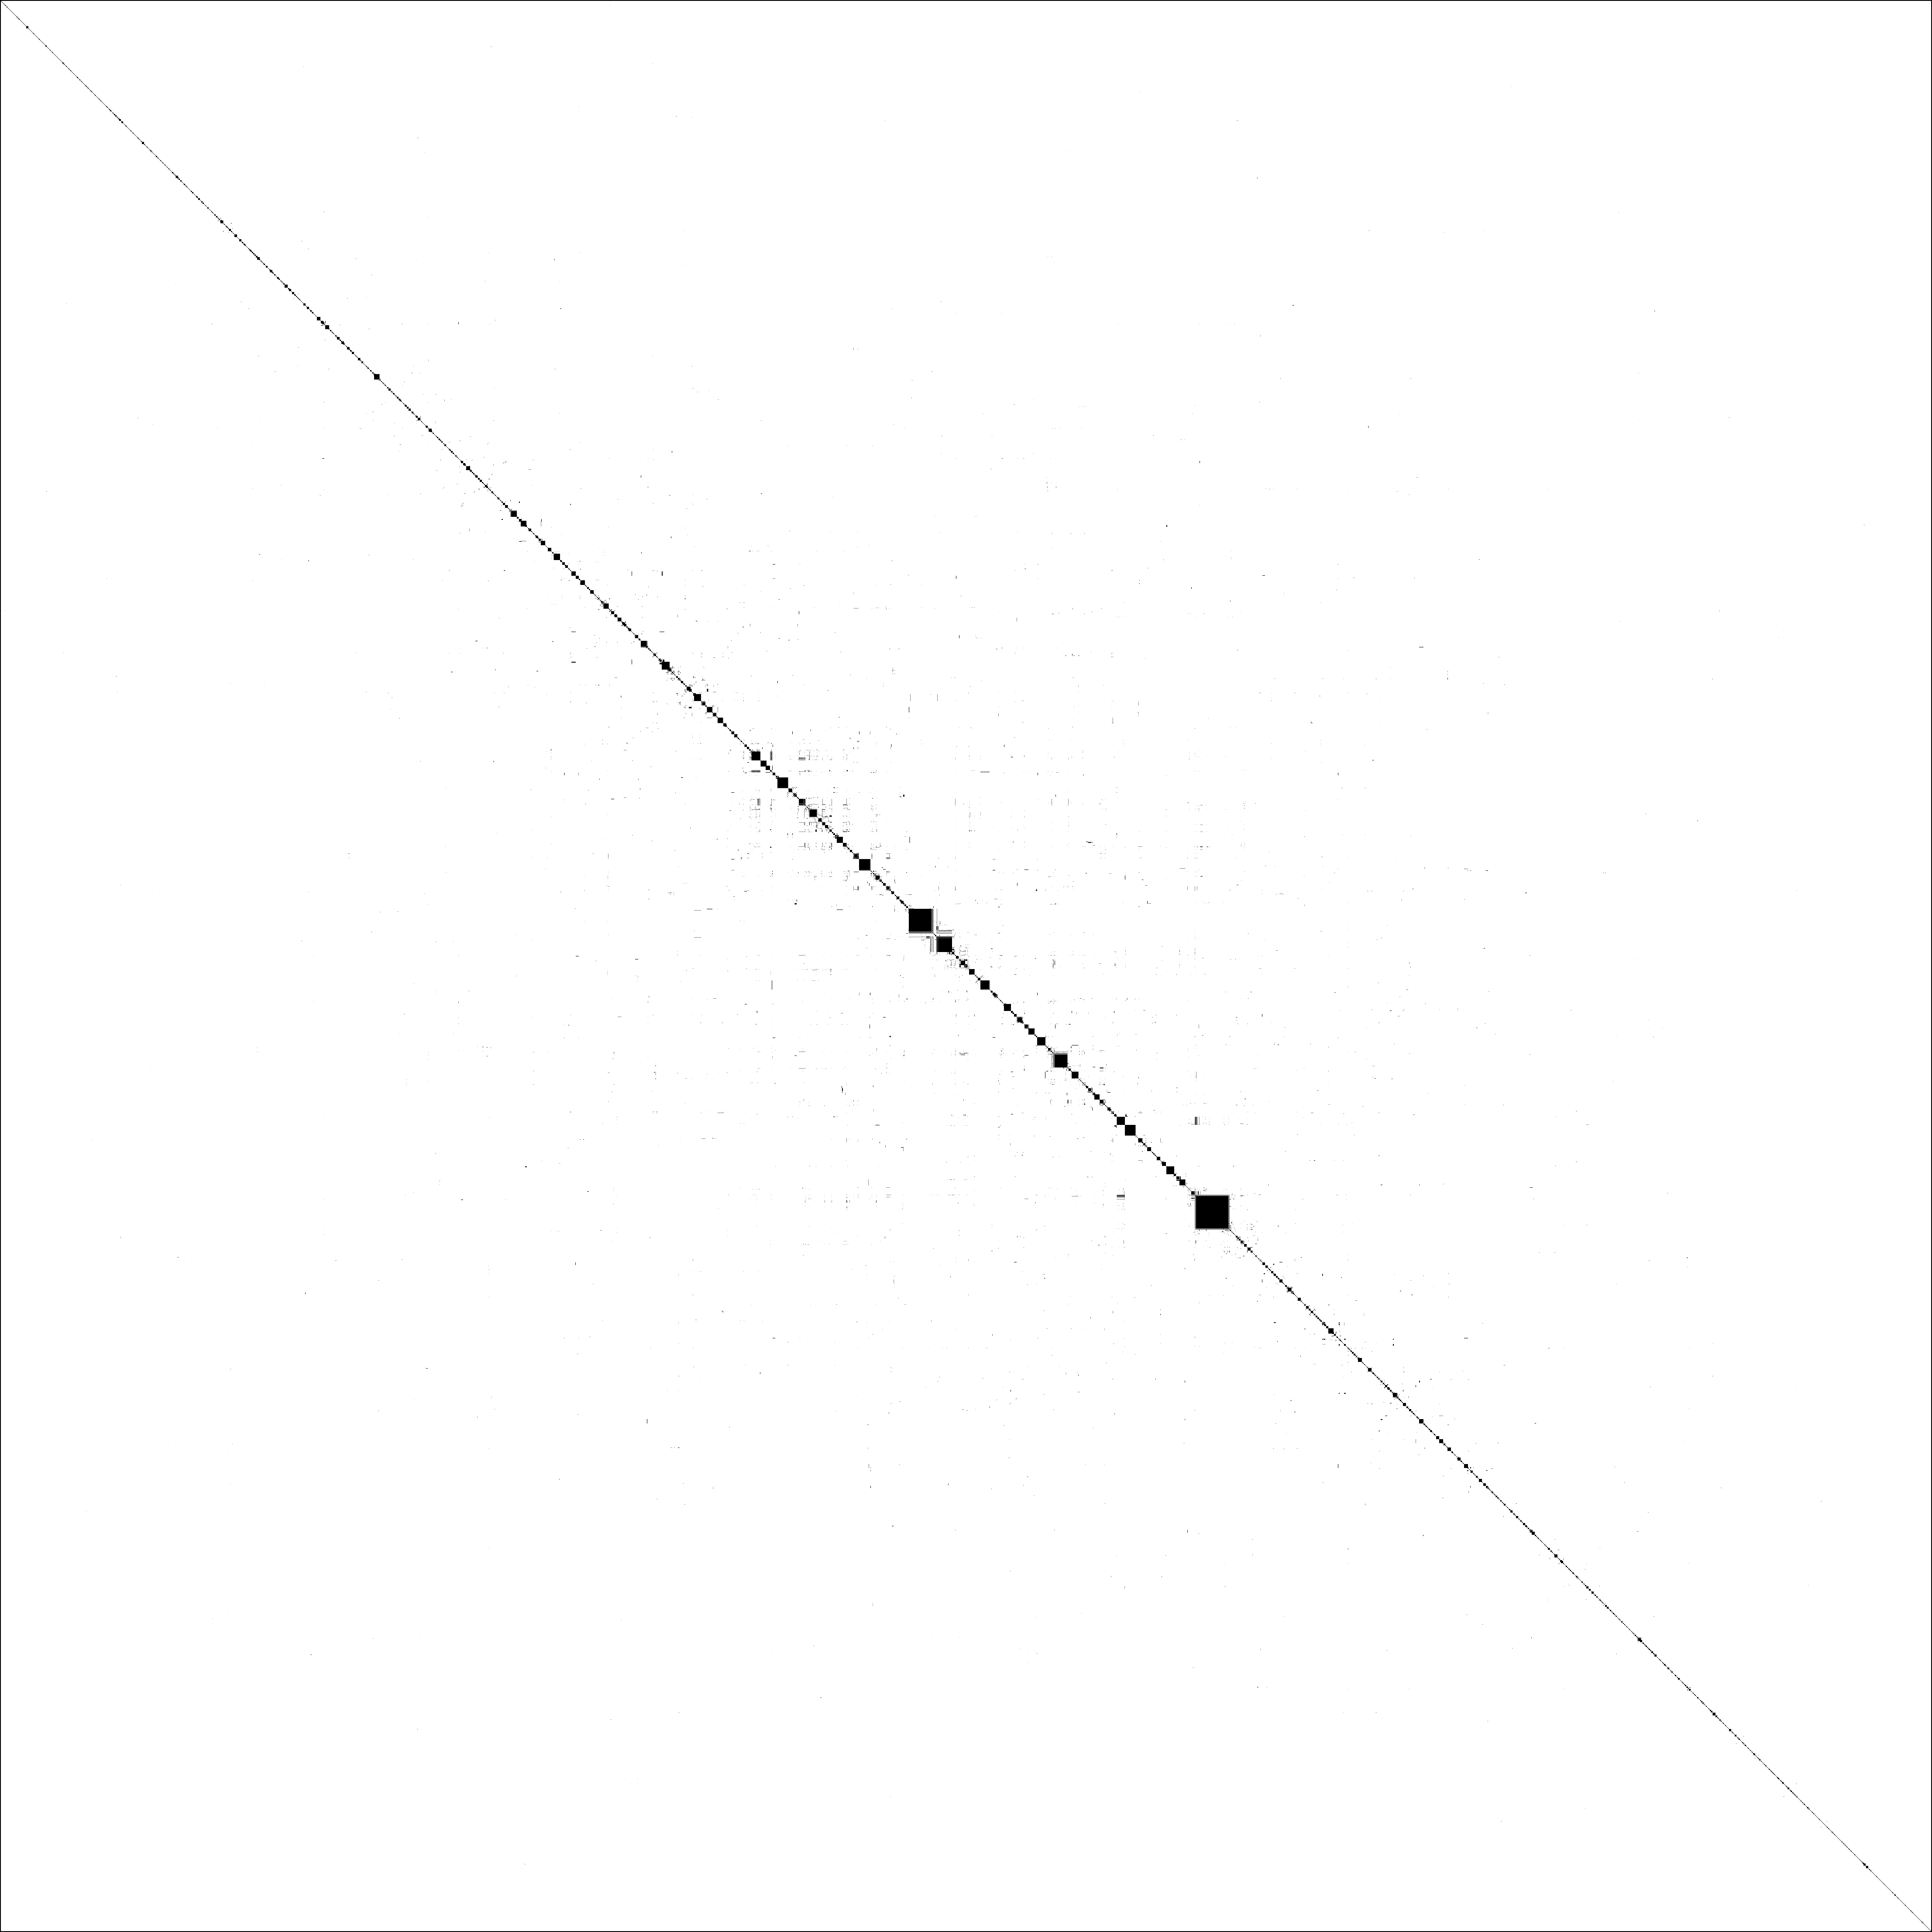
\includegraphics[width=\textwidth]{images/seed_94_step_0181.png}
    \caption{The most optimal solution of Algo. \ref{algo:gpu_hill_climbing} in 100 runs, with LA=0.06596.
    Computing this solution takes about 4 minutes.
    Now we can easily observe the structure of the research community.
    The largest square in the center represents the papers related to Yoshua Bengio;
    the second and third squares close to each other represents the papers related to Sergey Levine and Pieter Abbeel.
    Other clusters can be observed.
    }
    \label{fig:optimization_results}
\end{figure}

However, it still slightly suffers from local optima.
In order to get more globally optimal results, one can not rely on running the algorithm for longer.

Our best results are achieved by searching with 100 independent runs with random initialization.
However, we observe that the initial states matter more than trying different choices during optimization.
Thus, an evolutionary approach \cite{eppley2001} searching for better initial states might be better than our random initialization.
